\clearpage\section{Results}
\label{sec:experiments}

This chapter reports the experimental programme laid out in Section~\ref{sec:methodology}. It first walks the per-axis ablations one design axis at a time, establishing where accuracy comes from across the three tasks (Alzheimer's disease on ADReSSo, amyloid-$\beta$ status on SPIN, and PPA variant classification on the same SPIN subset), and then draws the strongest choices together into a best bundle for each task (Section~\ref{ssec:res_bytask}).

Two conventions hold throughout. ADReSSo is the only cohort with an official held-out partition, so it is the only task for which a \texttt{test-dist} accuracy is quoted alongside cross-validated validation accuracy; the two Spanish tasks are reported on validation folds only, and no artificial test split is ever substituted for the one they lack. Every accuracy is a mean over the five cross-validation folds and the two training seeds (43 and 3407), given as a point estimate. No significance testing was carried out, a limitation revisited in the conclusions (Section~\ref{sec:conclusions}).

Unless a table says otherwise, the numbers come from the unified \texttt{res\_model} implementation run under a single stable recipe (weighted Wav2Vec~2.0 layers, mean pooling, and no handcrafted features) so that one axis moves at a time. Where the older CogniAlign and DMHAM grids supply something the unified runs cannot, namely a second independent stack for the fusion and pooling trends or the legacy alignment sweep on amyloid, those numbers are brought in explicitly and labelled as such.

\subsection{Ablation findings}
\label{ssec:res_ablation}

The experiments isolate one design axis at a time, in the order the pipeline is built: which modalities to feed in, whether handcrafted features help, how to fuse the streams, how to pool the Wav2Vec layers, how to align audio to text, and which pretrained encoders to use. Each axis is varied with the others pinned to the stable recipe, so that a change in accuracy can be charged to the axis under test. For the two axes that a second, independent implementation also covers (fusion and Wav2Vec pooling), its agreement with the unified runs is noted. The per-task bundles these findings imply are gathered in Section~\ref{ssec:res_bytask}.

The modality axis comes first. Naive combination of the two streams is not enough. Concatenating or averaging the audio and text embeddings (Table~\ref{tab:res_modality}) never beats the better of the two unimodal branches, and on the Spanish tasks it sits well below it. The tasks also disagree about which modality carries the signal: amyloid is text-led (67.85\% text against 66.23\% audio), whereas PPA is audio-led (60.03\% against 53.57\%); ADReSSo, like amyloid, prefers text. The practical lesson is that extracting value from both modalities at once needs an attention-based fusion able to learn the correspondence between them. Simple pooling leaves accuracy on the table.

\begin{table}[htbp]
\centering
\caption[Modality ablation per task]{Modality ablation per task (\texttt{res\_model}). SPIN: weighted Wav2Vec~2.0 layers, mean pooling, no acoustic features, per-task default alignment. ADReSSo: minimal-encoder baselines, word$\rightarrow$token, final layer. Mean CV validation accuracy (\%) over seeds.}
\label{tab:res_modality}
\small
\begin{tabular}{lccc}
\toprule
 & \multicolumn{2}{c}{\textbf{SPIN}} & \textbf{ADReSSo} \\
\cmidrule(lr){2-3}\cmidrule(lr){4-4}
Input configuration & \textbf{Amyloid} & \textbf{PPA} & AD \\
\midrule
Audio only            & 66.23 & \textbf{60.03} & 53.97 \\
Text only             & \textbf{67.85} & 53.57 & \textbf{67.72} \\
Audio + Text (mean)   & 64.12 & 54.10 & 65.94 \\
Audio + Text (concat) & 64.12 & 54.10 & 65.94 \\
\bottomrule
\end{tabular}

\vspace{2pt}
{\footnotesize Unimodal branches dominate naive fusion; amyloid leans on text, PPA on audio. Attention fusion (Table~\ref{tab:res_fusion}) is required to exploit both modalities.}
\end{table}

Layered on top of those two streams are the handcrafted acoustic features. The 55 librosa/Praat descriptors are an optional side-channel, and the ablation (Table~\ref{tab:res_acoustic}) shows their contribution to be real but task-dependent. Concatenated after pooling, they lift amyloid by 2.1~pp (78.60\% to 80.68\%) and ADReSSo by 0.6~pp, but cost PPA 2.3~pp. There is no universal gain. That is why the recommended default leaves the features off and turns them on only where a task earns it, amyloid being the clear case, consistent with the pause- and voice-quality phenomenology of cognitive decline.

\begin{table}[htbp]
\centering
\caption[Handcrafted acoustic-feature ablation per task]{Handcrafted acoustic-feature (AF) ablation per task (\texttt{res\_model}, bidirectional cross-attention, weighted Wav2Vec~2.0 layers). 55-dim librosa/Praat descriptors. \emph{None} = no AF; \emph{token} = AF as an extra sequence token; \emph{concat} = AF concatenated after pooling. Mean CV validation accuracy (\%) over seeds. Per-task alignment: amyloid word$\rightarrow$token, PPA tok$\rightarrow$tok (uniform), ADReSSo word$\rightarrow$token.}
\label{tab:res_acoustic}
\small
\begin{tabular}{lccc}
\toprule
 & \multicolumn{2}{c}{\textbf{SPIN}} & \textbf{ADReSSo} \\
\cmidrule(lr){2-3}\cmidrule(lr){4-4}
Acoustic features & \textbf{Amyloid} & \textbf{PPA} & AD \\
\midrule
None              & 78.60 & \textbf{72.52} & 86.94 \\
Token integration & n/a$^{\ast}$ & n/a$^{\ast}$ & 86.94 \\
Concatenation     & \textbf{80.68} & 70.25 & \textbf{87.54} \\
\bottomrule
\end{tabular}

\vspace{2pt}
{\footnotesize $^{\ast}$Token-level AF integration was only swept on ADReSSo. Concatenated AF helps ADReSSo ($+0.6$~pp) and amyloid ($+2.1$~pp) but slightly hurts PPA ($-2.3$~pp): acoustic features are beneficial but task-dependent, not universal.}
\end{table}

With the inputs settled, the central axis is how to fuse them. Fusion is the axis with the widest spread (Table~\ref{tab:res_fusion}, shown graphically in Figure~\ref{fig:res_fusion_bar}), and the three groups behave exactly as their inductive biases would predict. The two non-sequential baselines and plain self-attention stay near chance on the Spanish tasks; self-attention over an undifferentiated audio--text bag has no way to find the cross-modal structure on its own. Positional information and multiple heads help, but the decisive jump comes from keeping the modalities apart and letting one attend to the other. The cross-attention family (plain, gated, and bidirectional) tops every task: between 81 and 83\% on amyloid, the low seventies on PPA, and the high eighties on ADReSSo. Mamba is the telling outlier. It is strong on English and amyloid (85.40\% on ADReSSo, 77.49\% on amyloid) yet collapses to 52.57\% on PPA, and that collapse is what rules it out as a general-purpose default despite its ADReSSo standing.

\begin{figure}[htbp]
\centering
\resizebox{\linewidth}{!}{%
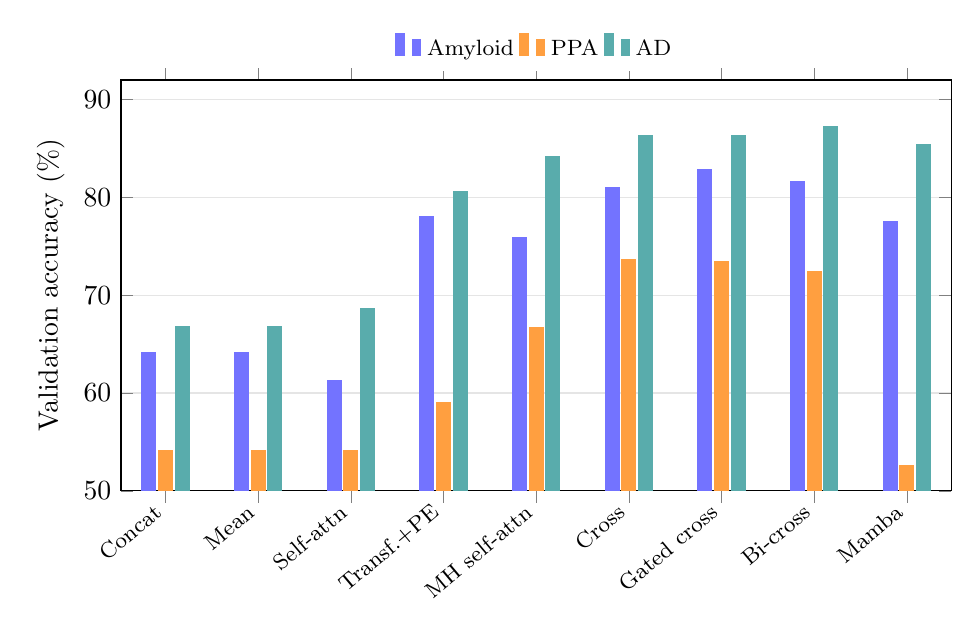
\begin{tikzpicture}
\begin{axis}[
    width=\linewidth, height=6.8cm,
    ybar=1pt, bar width=5pt,
    ymin=50, ymax=92,
    ylabel={Validation accuracy (\%)},
    ylabel near ticks,
    symbolic x coords={Concat,Mean,Self-attn,Transf.+PE,MH self-attn,Cross,Gated cross,Bi-cross,Mamba},
    xtick=data,
    x tick label style={rotate=40,anchor=east,font=\footnotesize},
    ytick={50,60,70,80,90},
    enlarge x limits=0.06,
    ymajorgrids, grid style={gray!20},
    legend style={at={(0.5,1.02)},anchor=south,legend columns=3,font=\footnotesize,draw=none},
]
\addplot[fill=blue!55,draw=blue!55] coordinates {(Concat,64.12)(Mean,64.12)(Self-attn,61.26)(Transf.+PE,78.05)(MH self-attn,75.85)(Cross,81.00)(Gated cross,82.88)(Bi-cross,81.64)(Mamba,77.49)};
\addplot[fill=orange!75,draw=orange!75] coordinates {(Concat,54.10)(Mean,54.10)(Self-attn,54.09)(Transf.+PE,59.04)(MH self-attn,66.66)(Cross,73.67)(Gated cross,73.46)(Bi-cross,72.43)(Mamba,52.57)};
\addplot[fill=teal!65,draw=teal!65] coordinates {(Concat,66.83)(Mean,66.83)(Self-attn,68.65)(Transf.+PE,80.58)(MH self-attn,84.22)(Cross,86.34)(Gated cross,86.34)(Bi-cross,87.23)(Mamba,85.40)};
\legend{Amyloid, PPA, AD}
\end{axis}
\end{tikzpicture}%
}
\caption[Fusion-family accuracy across tasks]{Validation accuracy of the fusion families on the three tasks (values from Table~\ref{tab:res_fusion}). The cross-attention family leads on every task, while Mamba's drop to chance on PPA stands out as the clearest outlier. Abbreviations: \emph{Concat}~=~concatenation, \emph{Mean}~=~element-wise mean (both non-sequential baselines); \emph{Self-attn}~=~self-attention, \emph{MH self-attn}~=~multi-head self-attention, \emph{Transf.+PE}~=~transformer with positional encoding; \emph{Cross}~=~cross-attention, \emph{Gated cross}~=~gated cross-attention, \emph{Bi-cross}~=~bidirectional cross-attention; \emph{Mamba}~=~selective state-space fusion.}
\label{fig:res_fusion_bar}
\end{figure}

This ranking is the main trend the second, independent DMHAM stack was built to check, and it survives the change of implementation. In the legacy fusion grid the cross-attention and Mamba families again lead within DMHAM (bidirectional cross-attention reaches 85.21\% validation on ADReSSo, for instance), even though DMHAM uses different encoders, a different ASR path, and a shorter training schedule. The absolute numbers diverge between the two stacks, which are not a controlled head-to-head, but the ordering of fusion families holds, and reproducing that ordering twice is the whole point of running it twice. Inference cost is not a discriminating factor among the families: with the encoder outputs precomputed and cached, every fusion variant runs in well under a millisecond per sample, so the choice is driven by accuracy alone.

\begin{table}[htbp]
\centering
\caption[Fusion-technique ablation per task]{Fusion-technique ablation per task (\texttt{res\_model}, weighted Wav2Vec~2.0 layers, no acoustic features). The first two rows (concatenation, element-wise mean) are non-sequential baselines; the remaining seven are the sequence-to-sequence fusion families of Table~\ref{tab:fusion}. Mean CV validation accuracy (\%) over seeds. Fixed per-task alignment: ADReSSo tok$\rightarrow$tok (char); amyloid word$\rightarrow$token; PPA tok$\rightarrow$tok (uniform).}
\label{tab:res_fusion}
\small
\begin{tabular}{lccc}
\toprule
 & \multicolumn{2}{c}{\textbf{SPIN}} & \textbf{ADReSSo} \\
\cmidrule(lr){2-3}\cmidrule(lr){4-4}
Fusion technique & \textbf{Amyloid} & \textbf{PPA} & AD \\
\midrule
Concatenation                 & 64.12 & 54.10 & 66.83 \\
Element-wise mean             & 64.12 & 54.10 & 66.83 \\
Self-attention                & 61.26 & 54.09 & 68.65 \\
Transformer (positional)      & 78.05 & 59.04 & 80.58 \\
Multi-head self-attention     & 75.85 & 66.66 & 84.22 \\
Cross-attention               & 81.00 & \textbf{73.67} & 86.34 \\
Gated cross-attention         & \textbf{82.88} & 73.46 & 86.34 \\
Bidirectional cross-attention & 81.64 & 72.43 & \textbf{87.23} \\
Mamba                         & 77.49 & 52.57 & 85.40 \\
\bottomrule
\end{tabular}

\vspace{2pt}
{\footnotesize Cross-attention variants dominate on every task; Mamba is competitive on English and amyloid but collapses on PPA. The concatenation and element-wise-mean baselines, and plain self-attention, stay near chance on SPIN. The two baselines also appear in the modality study (Table~\ref{tab:res_modality}); the small ADReSSo difference reflects the minimal head used there versus the full per-task recipe used here.}
\end{table}

With a fusion mechanism chosen, attention turns back to the audio branch. Two questions sit on it: whether to read the final Wav2Vec layer or a learnable mixture of all twelve, and, if a mixture, whether a single global set of weights is enough. The pooling table (Table~\ref{tab:res_wav2vec_pool}) gives a muted answer. A weighted layer stack helps ADReSSo slightly (86.64\% against 86.32\%), but on the Spanish tasks the final layer is as good or better, clearly so on PPA (74.95\% against 72.43\%). Depth, once a competent fusion is in place, buys little.

The adaptive layer mixer, evaluated only in the unified implementation, sharpens the picture. Replacing the single global weight vector with a per-utterance \emph{sample} mixer at temperature 0.1 lifts ADReSSo from 87.23\% (global mixer, uniform initialisation) to \textbf{88.16\%}, and the learned weights are interpretable: the mixer concentrates on the top layer (layer~11, weight $\approx 0.20$ against the uniform 0.083) while keeping secondary mass on the lowest layer, and it varies those weights from one utterance to the next instead of settling on a single profile (Figure~\ref{fig:res_layer_mixer}). The finer \emph{token} mixer does not improve on this, so the per-utterance sample mixer is the variant carried into the recommendation: cheap, input-conditioned, and biased toward the upper layers where lexical content concentrates.

\begin{figure}[htbp]
\centering
\resizebox{\linewidth}{!}{%
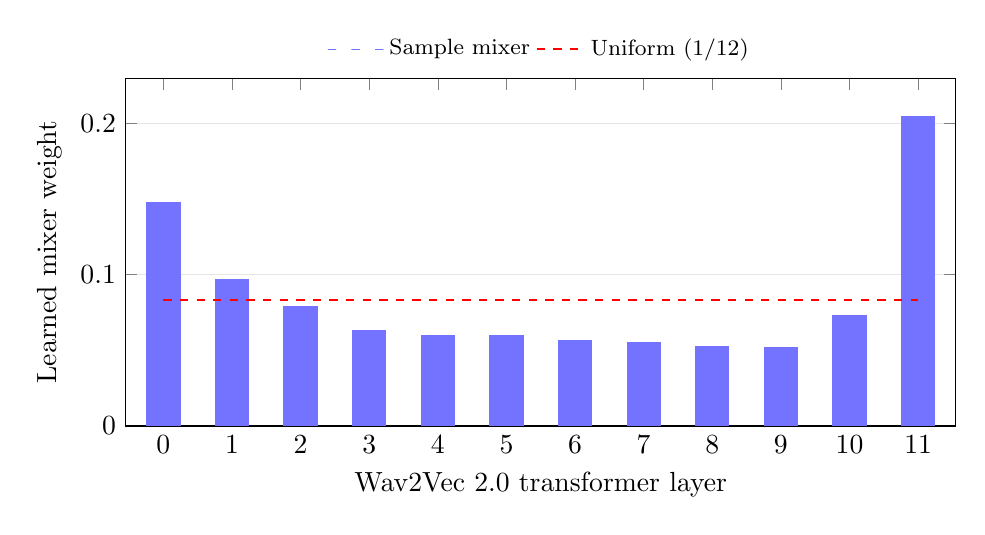
\begin{tikzpicture}
\begin{axis}[
    width=\linewidth, height=6cm,
    ylabel={Learned mixer weight},
    xlabel={Wav2Vec~2.0 transformer layer},
    symbolic x coords={0,1,2,3,4,5,6,7,8,9,10,11},
    xtick=data,
    ymin=0, ymax=0.23,
    enlarge x limits=0.05,
    ymajorgrids, grid style={gray!20},
    legend style={at={(0.5,1.02)},anchor=south,legend columns=2,font=\footnotesize,draw=none},
]
\addplot[ybar, bar width=12pt, fill=blue!55, draw=blue!55] coordinates {
    (0,0.1478)(1,0.0970)(2,0.0788)(3,0.0634)(4,0.0596)(5,0.0597)(6,0.0568)(7,0.0554)(8,0.0523)(9,0.0517)(10,0.0731)(11,0.2046)};
\addplot[red, dashed, thick, mark=none] coordinates {(0,0.0833)(11,0.0833)};
\legend{Sample mixer, Uniform ($1/12$)}
\end{axis}
\end{tikzpicture}%
}
\caption[Learned layer-mixer weights]{Learned per-layer weights of the per-utterance sample mixer on ADReSSo (seed~43, $\tau = 0.1$, twelve Wav2Vec~2.0 layers). Weight concentrates on the uppermost layer (layer~11) and, secondarily, the lowest, both well above the uniform $1/12$ baseline (dashed); the mean per-utterance spread of these weights is $0.24$.}
\label{fig:res_layer_mixer}
\end{figure}

\begin{table}[htbp]
\centering
\caption[Wav2Vec layer-pooling ablation per task]{Wav2Vec~2.0 layer-pooling ablation per task (\texttt{res\_model}, bidirectional cross-attention). \emph{Final} = last layer; \emph{weighted} = learnable 12-layer mixture. Mean CV validation accuracy (\%) over seeds. Per-task alignment: amyloid tok$\rightarrow$tok (char), PPA tok$\rightarrow$tok (uniform), ADReSSo word$\rightarrow$token.}
\label{tab:res_wav2vec_pool}
\small
\begin{tabular}{lccc}
\toprule
 & \multicolumn{2}{c}{\textbf{SPIN}} & \textbf{ADReSSo} \\
\cmidrule(lr){2-3}\cmidrule(lr){4-4}
Pooling & \textbf{Amyloid} & \textbf{PPA} & AD \\
\midrule
Final layer     & \textbf{80.75} & \textbf{74.95} & 86.32 \\
Weighted layers & 80.75 & 72.43 & \textbf{86.64} \\
\bottomrule
\end{tabular}

\vspace{2pt}
{\footnotesize Weighted layers help ADReSSo slightly; on SPIN the final layer is as good or better, especially on PPA.}
\end{table}

The next axis, audio--text alignment, is the thesis's own contribution, so it is examined under two lenses. Under the unified stable recipe (Table~\ref{tab:res_alignment}) the three schemes finish close together on all three tasks: character-proportional token-to-token is best on PPA (73.48\%), word-to-token edges amyloid (81.64\%), and on ADReSSo the two token-to-token schemes and the baseline are within a few tenths of a point. Subword alignment is therefore not a free lunch under every configuration, and that is worth stating plainly.

The larger effect appears in the configuration where it should: the legacy alignment grid on amyloid, with handcrafted features and a final-layer audio representation. There, character-proportional alignment reaches 85.72\% against 85.13\% for word-to-token, with the uniform scheme matching the baseline at 85.13\%. The proportional allocation, which gives longer subwords proportionally more of the spoken word's acoustic frames, is the one refinement that helps, and amyloid is where it helps most. Read across both lenses, the honest summary is that token-to-token alignment is a worthwhile, low-cost refinement that pays off on specific task and feature combinations rather than a universal improvement, and that the character-proportional variant is the stronger of the two proposals.

\begin{table}[htbp]
\centering
\caption[Audio--text alignment ablation per task]{Audio--text alignment ablation per task (\texttt{res\_model}, bidirectional cross-attention, weighted Wav2Vec~2.0 layers). Mean CV validation accuracy (\%) over seeds. The token$\rightarrow$token schemes are the contribution of this thesis.}
\label{tab:res_alignment}
\small
\begin{tabular}{llccc}
\toprule
 & & \multicolumn{2}{c}{\textbf{SPIN}} & \textbf{ADReSSo} \\
\cmidrule(lr){3-4}\cmidrule(lr){5-5}
Alignment & Source & \textbf{Amyloid} & \textbf{PPA} & AD \\
\midrule
word$\rightarrow$token        & CogniAlign  & \textbf{81.64} & 72.43 & \textbf{86.32} \\
tok$\rightarrow$tok (uniform) & This thesis & 79.79 & 72.43 & 86.02 \\
tok$\rightarrow$tok (char)    & This thesis & 80.75 & \textbf{73.48} & 86.02 \\
\bottomrule
\end{tabular}

\vspace{2pt}
{\footnotesize Under a stable recipe the three alignments are close on all tasks; character-proportional token$\rightarrow$token is best on PPA, while word$\rightarrow$token edges amyloid. The larger token$\rightarrow$token gain on amyloid appears in the legacy AF + final-layer stack, where the proportional scheme reaches 85.72\%.}
\end{table}

The last axis swaps the pretrained encoders one at a time (Table~\ref{tab:res_encoder}), and the outcome is firmly task-dependent. ADReSSo is best served by the original lightweight pairing of DistilBERT text with the English Wav2Vec~2.0 base encoder (86.12\%), and degrades when either is replaced, most sharply when the audio encoder switches to the multilingual XLSR-300M (80.37\%). The Spanish tasks pull the other way: XLSR-300M audio gives amyloid its best encoder result (81.40\%), and ModernBERT text helps PPA (71.70\%). The larger cross-lingual audio model earns its place precisely where the language no longer matches the English pretraining, which is the contrast the ablation was designed to expose, and a reminder that the most capable encoder is not automatically the right one once the task is fixed.

\begin{table}[htbp]
\centering
\caption[Feature-extractor single-factor ablation per task]{Feature-extractor (encoder) single-factor ablation per task (\texttt{res\_model}; fixed recipe: bidirectional cross-attention, word$\rightarrow$token, weighted Wav2Vec~2.0 + sample mixer). One component swapped per run; mean CV validation accuracy (\%) over seeds 43 and 3407.}
\label{tab:res_encoder}
\small
\begin{tabular}{lllccc}
\toprule
 & & & \multicolumn{2}{c}{\textbf{SPIN}} & \textbf{ADReSSo} \\
\cmidrule(lr){4-5}\cmidrule(lr){6-6}
Variant & Text encoder & Audio encoder & \textbf{Amyloid} & \textbf{PPA} & AD \\
\midrule
Baseline              & DistilBERT & Wav2Vec2 base-960h & 79.84 & 69.94 & \textbf{86.12} \\
Audio $\to$ XLSR      & DistilBERT & Wav2Vec2 XLSR-300M & \textbf{81.40} & 71.68 & 80.37 \\
Text $\to$ ModernBERT & ModernBERT & Wav2Vec2 base-960h & 81.36 & \textbf{71.70} & 77.38 \\
Text $\to$ BERT       & BERT-base  & Wav2Vec2 base-960h & 79.88 & 69.93 & 81.91 \\
\bottomrule
\end{tabular}

\vspace{2pt}
{\footnotesize ADReSSo favours DistilBERT + base-960h; on SPIN, XLSR-300M audio (amyloid) and ModernBERT text (PPA) slightly exceed the baseline.}
\end{table}

\subsection{Results by task}
\label{ssec:res_bytask}

Taken as a whole, the unified \texttt{res\_model} runs reproduce the main trends established on the two primitive stacks (the cross-attention family wins fusion, depth beyond the final layer adds little, and subword alignment helps narrowly and task-specifically), while adding the two studies the primitive stacks could not express cleanly: the adaptive layer mixer and the single-factor encoder swaps. The grid does not point to one winning configuration but to a different best bundle for each task, collected in Table~\ref{tab:res_best}. No two of them share the same recipe, which is the thesis's central empirical message in miniature: the best choice along each axis depends on the task, and a single configuration that wins everywhere does not exist in this grid. What the evidence supports instead is a sensible cross-task default, bidirectional cross-attention, word-to-token alignment, a weighted audio stack with the sample mixer, and handcrafted features off, that stays close to each per-task best while remaining stable across folds, seeds, and tasks. The three bundles are read out below.

\textbf{Alzheimer's disease (ADReSSo).} ADReSSo is the anchor task and the only one with an official held-out partition, so it is the one place a model is judged on a previously unseen split rather than on its own folds. The recommended configuration, bidirectional cross-attention over word-to-token-aligned streams with a weighted Wav2Vec stack refined by the per-utterance sample mixer, reaches \textbf{88.16\%} validation accuracy, obtained without leaderboard-specific tuning. The official \texttt{test-dist} partition tells a complementary story: the Mamba block edges the validation grid (88.44\%) and, run through the full-training protocol, reaches \textbf{83.10\%} on that held-out split, among the stronger challenge systems and the only configuration evaluated there. That is a genuine finding; but because the same block collapses on PPA and its ADReSSo lead is seed-sensitive, the recommendation keeps the steadier bidirectional cross-attention.

\textbf{Amyloid-$\beta$ status (SPIN).} The amyloid task recovers a fluid biomarker from forty seconds of Spanish picture description, with no official test set, so every figure is a five-fold cross-validation accuracy. It leans on the text stream (Table~\ref{tab:res_modality}), and gated cross-attention is the best plain fusion at 82.88\%. Its headline comes from the configuration the thesis contributes: character-proportional token-to-token alignment, a final-layer audio representation, bidirectional cross-attention, and the 55 handcrafted features switched on, reaching \textbf{83.90\%}. Amyloid is also where the alignment contribution shows most clearly: in the legacy handcrafted-feature and final-layer grid the proportional scheme reaches 85.72\% against 85.13\% for word-to-token, the largest of the alignment gains.

\textbf{PPA variant (SPIN).} PPA is the hardest task, a three-class problem over a small, imbalanced cohort whose fold-level accuracy is noisy, so its numbers are read as indicative rather than definitive. The best bundle, bidirectional cross-attention with uniform token-to-token alignment and a final-layer audio representation, reaches \textbf{74.95\%}. PPA is the only task that prefers audio to text as a single modality (60.03\% against 53.57\%), consistent with the motor-speech and fluency disturbances of the non-fluent variant, and the only one that punishes the wrong fusion outright, with the Mamba block falling to 52.57\%, barely above the majority class.

\begin{table}[htbp]
\centering
\caption[Best technique bundle per task]{Best technique bundle per task in the unified \texttt{res\_model} implementation. SPIN (amyloid, PPA) are Spanish, 5-fold CV validation only; ADReSSo (English) additionally reports official test-dist accuracy after full training. Mean over seeds 43 and 3407.}
\label{tab:res_best}
\small
\begin{tabular}{llcc}
\toprule
Task & Best technique stack & Val.\ acc.\ (\%) & Test acc.\ (\%) \\
\midrule
\textbf{Amyloid (SPIN)} & bicross, tok$\rightarrow$tok (char), final Wv, $+$AF & \textbf{83.90}$^{a}$ & n/a \\
\textbf{PPA (SPIN)}     & bicross, tok$\rightarrow$tok (uniform), final Wv & \textbf{74.95} & n/a \\
AD (ADReSSo, ref.)      & Mamba, word$\rightarrow$token, final Wv & 88.44 & 83.10$^{b}$ \\
\bottomrule
\end{tabular}

\vspace{2pt}
{\footnotesize $^{a}$Best single run (seed 43, lr $1.5\times10^{-5}$, dropout 0.25) with the 55-d handcrafted acoustic features; the plain-recipe gated cross-attention reaches 82.88\%. $^{b}$Official ADReSSo test-dist under the full-train protocol. Mamba tops the ADReSSo grid, but the recommended cross-task default is bidirectional cross-attention with the per-utterance sample mixer (88.16\% cross-validated validation accuracy), preferred for its stability across all three tasks rather than its single-task peak.}
\end{table}

\subsection{Error Analysis}
\label{ssec:res_error}

A detailed error analysis, including per-class confusion matrices for the three-class PPA task and an inspection of misclassified ADReSSo and amyloid cases, is left as future work. The present study reports point-estimate accuracies without confusion-level breakdowns or significance testing; characterising systematic failure modes, for example confusion between the logopenic and non-fluent PPA variants or the influence of ASR transcription errors on the text stream, would require the per-sample prediction logs and is identified here as a direction for subsequent analysis rather than reported with fabricated figures.
